\subsection{Newton Polynomials}

\frame{
\begin{itemize}
\item It is sometimes useful to find several approximating polynomials $P_1(X)$, $P_2(X)$, $\ldots$, $P_N(x)$ and then choose the one that suits our needs. 
\item If the Lagrange polynomials are used, there is no constructive relationship between $P_{N-1}(X)$ and $P_N(X)$.
\item Each polynomial has to be constructed individually, and the work required to compute the higher-degree polynomials involves many computations. 
\end{itemize}
}

\frame{
We take a new approach and construct Newton polynomials that have the recursive pattern 
\begin{equation*}
\begin{array}{l c l}
P_1(x) & = & a_0 + a_1(x - x_0), \\
P_2(x) & = & a_0 + a_1(x - x_0) + a_2(x - x_0)(x - x_1), \\
P_3(x) & = & a_0 + a_1(x - x_0) + a_2(x - x_0)(x - x_1) \\
& & + a_3(x - x_0)(x - x_1)(x - x_2), \\
& \vdots & \\
P_N (x) & = & a_0 + a_1(x - x_0) + a_2(x - x_0)(x - x_1) \\
& & + a_3(x - x_0)(x - x_1)(x - x_2) \\
& & + a_4(x - x_0)(x - x_1)(x - x_2)(x - x_3) + \cdots \\
& & + a_N (x - x_0) \cdots (x - x_{N-1}).
\end{array}
\end{equation*}
}

\frame{
Here the polynomial $P_N(x)$ is obtained from $P_{N-1}(X)$ using the recursive relationship
\begin{equation*}
P_N (x) = P_{N-1}(x) + a_N (x - x_0)(x - x_1)(x - x_2) \cdots (x - x_{N-1}).
\end{equation*}
The polynomial (3.60) is said to be a Newton polynomial with $N$ centers $x_0$, $x_1$, $\ldots$, $x_{N-1}$. 
It involves sums of products of linear factors up to 
\begin{equation*}
a_N (x - x_0)(x - x_1)(x - x_2) \cdots (x - x_{N-1}),
\end{equation*}
so $P_N(x)$ will simply be an ordinary polynomial of degree $\le N$. 
}

\frame{
\frametitle{Example.}
Given the centers $x_0 = 1$, $x_1 = 3$, $x_2 = 4$, and $x_3 = 4.5$ and the coefficients $a_0 = 5$, $a_1 = -2$, $a_2 = 0.5$, $a_3 = -0.1$, and $a_4 = 0.003$, find $P_1(x)$, $P_2(x)$, $P_3(x)$, and $P_4(x)$ and evaluate $P_k (2.5)$ for $k = 1, 2, 3, 4$.
\begin{center}
$\Downarrow$
\end{center}
Using the recursive pattern formulas introduced above, we have
\begin{equation*}
\begin{array}{l c l}
P_1(x) & = & 5 - 2(x - 1), \\
P_2(x) & = & P_1(x) + 0.5(x - 1)(x - 3), \\
P_3(x) & = & P_2(x) - 0.1(x - 1)(x - 3)(x - 4), \\
P_4(x) & = & P_3(x) + 0.003(x - 1)(x - 3)(x - 4)(x - 4.5).
\end{array}
\end{equation*}
Evaluating the polynomials at $x = 2.5$ results in
\begin{equation*}
\begin{array}{l c l}
P_1(2.5) & = & 5 - 2(1.5) = 2, \\
P_2(2.5) & = & P_1(2.5) + 0.5(1.5)(-0.5) = 1.625, \\
P_3(2.5) & = & P_2(2.5) - 0.1(1.5)(-0.5)(-1.5) = 1.5125, \\
P_4(2.5) & = & P_3(2.5) + 0.003(1.5)(-0.5)(-1.5)(-2.0) = 1.50575.
\end{array}
\end{equation*}
}

\frame{
\frametitle{Nested Multiplication}
\begin{itemize}
\item If $N$ is fixed and the polynomial $P_N(x)$ is evaluated many times, then nested multiplication should be used. 
\item The process is similar to nested multiplication for ordinary polynomials, except that the centers $x_k$ must be subtracted from the independent variable $x$. 
\item The nested multiplication form for $P_3(x)$ is 
\end{itemize}
\begin{equation*}
P_3(x) = ((a_3(x - x_2) + a_2)(x - x_1) + a_1)(x - x_0) + a_0.
\end{equation*}
To evaluate $P_3(x)$ for a given value of $x$, start with the innermost grouping and form successively the quantities 
\begin{equation*}
\begin{array}{l c l}
S_3 & = & a_3, \\
S_2 & = & S_3(x - x_2) + a_2, \\
S_1 & = & S_2(x - x_1) + a_1, \\
S_0 & = & S_1(x - x_0) + a_0. 
\end{array}
\end{equation*}
The quantity $S_0$ is now $P_3(x)$.
}

\frame{
\frametitle{Example}
Compute P3(2.5) in Example 3.10 using nested multiplication.
\begin{center}
$\Downarrow$
\end{center}
\begin{equation*}
P_3(x) = ((-0.1(x - 4) + 0.5)(x - 3) - 2)(x - 1) + 5.
\end{equation*}
The values  are
\begin{equation*}
\begin{array}{l c l}
S_3 & = & -0.1, \\
S_2 & = & -0.1(2.5 - 4) + 0.5 = 0.65, \\
S_1 & = & 0.65(2.5 - 3) - 2 = -2.325, \\
S_0 & = & -2.325(2.5 - 1) + 5 = 1.5125.
\end{array}
\end{equation*}
}

\frame{
\frametitle{Polynomial Approximation, Nodes, and Centers}
\begin{itemize}
\item Suppose that we want to find the coefficients ak for all the polynomials $P_1(x)$, $\ldots$ , $P_N(x)$ that approximate a given function $f(x)$. 
\item Then $P_k(X)$ will be based on the centers $x_0$, $x_1$, $\ldots$, $x-k$ and have the nodes $x-0$, $x_1$, $\ldots$, $x_{k+1}$. 
\item For the polynomial $P_1(x)$ the coefficients ao and al have a familiar meaning. 
\end{itemize}
}

\frame{
In this case 
\begin{equation*}
P_1(x_0) = f (x_0) \ \ \ and \ \ \ P_1(x_1) = f (x_1).
\end{equation*}
%Using (3.57) and (3.64) to solve for ao, we find that 
\begin{equation*}
f (x_0) = P_1(x_0) = a_0 + a_1(x_0 - x_0) = a_0.
\end{equation*}
Hence $a_0 = f(x_0)$. 
%Next, using (3.57), (3.64), and (3.65), we have
\begin{equation*}
f (x_1) = P_1(x_1) = a_0 + a_1(x_1 - x_0) = f (x_0) + a_1(x_1 - x_0),
\end{equation*}
which can be solved for $a_1$, and we get
\begin{equation*}
a_1 = \frac{f (x_1) - f (x_0)}{x_1 - x_0}
\end{equation*}
Hence $a_1$ is the slope of the secant line passing through the two points $(x_0,f(x_0))$ and $(x_1,f(x_1))$ 
}

\frame{
The coefficients $a_0$ and $a_1$ are the same for both $P_1 (X)$ and $P_2(x)$. 
%Evaluating (3.58) at the node $x_2$, we find that 
\begin{equation*}
f (x_2) = P_2(x_2) = a_0 + a_1(x_2 - x_0) + a_2(x_2 - x_0)(x_2 - x_1).
\end{equation*}
The values for $a_0$ and $a_1$ in (3.65) and (3.66) can be used in (3.67) to obtain
\begin{equation*}
\begin{array}{l c l}
a_2 & = & \frac{ f (x_2) - a_0 - a_1(x_2 - x_0)}{(x_2 - x_0)(x_2 - x_1)} \\
 & & = \left(  \frac{f (x_2) - f (x_0)}{x_2 - x_0} - \frac{f (x_1) - f (x_0)}{x_1 - x_0}  \right)
\slash \left( x_2 - x_1 \right)
\end{array}
\end{equation*}
For computational purposes we prefer to write this last quantity as
\begin{equation*}
a_2 = \left(  \frac{f (x_2) - f (x_1)}{x_2 - x_1} - \frac{f (x_1) - f (x_0)}{x_1 - x_0}  \right) \slash \left( x_2 - x_0 \right).
\end{equation*}
}

\frame{
\begin{itemize}
\item The two formulas for $a_2$ can be shown to be equivalent by writing the quotients over the common denominator $(x_22 - x_1l)(x_2 - x_0)(x-1 - x_0)$. 
\item The details are left for the reader. 
%\item The numerator in (3.68) is the difference between the first-order divided differences. 
\item In order to proceed, we need to introduce the idea of divided differences. 
\end{itemize}
}

\frame{
\begin{block}{Definition }
 The divided differences for a function f (x) are defined as follows:
\begin{equation*}
\begin{array}{r c l}
f [x_k] & = & f (x_k ) \\
f [x_{k-1}, x_k] & = & \frac{f [x_k] - f [x_{k-1}]}{x_k - x_{k-1}} \\
f [x_{k-2}, x_{k-1}, x_k] & = & \frac{ f [x_{k-1}, x_k] - f [x_{k-2}, x_{k-1}]}{x_k - x_{k-2}} \\
f [x_{k-3}, x_{k-2}, x_{k-1}, x_k] & = & \frac{f [x_{k-2}, x_{k-1}, x_k] - f [x_{k-3}, x_{k-2}, x_{k-1}]}{x_k - x_{k-3}}
\end{array}
\end{equation*}
The recursive rule for constructing higher-order divided differences is
\begin{equation*}
f [x_{k-j} , x_{k-j+1}, \ldots, x_k] = \frac{ f [x_{k-j+1}, \ldots, x_k] - f [x_{k-j} , \ldots, x_{k-1}]}{x_k - x_{k-j}}
\end{equation*}
and is used to construct the divided differences in the Divided-Difference Table. 
\end{block}
}

\frame{
\begin{figure}
\begin{center}
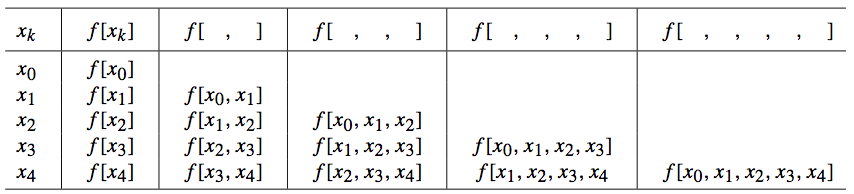
\includegraphics[width=100mm]{chap-3/tab_4-8.png}
\end{center}
\end{figure} 
The coefficients $a_k$ of $P_N(x)$ depend on the values $f(x_j)$, for $j = 0$, $1$, $\ldots$, $k$. 
The next theorem shows that ak can be computed using divided differences: 
\begin{equation*}
a_k = f [x_0, x_1, \ldots, x_k ].
\end{equation*}
}

\frame{
\begin{block}{Theorem  (Newton Polynomial).}
Suppose that $x_0$, $x_1$, $\ldots$, $x_N$ are $N +1$ distinct numbers in $[a, b]$. 
There exists a unique polynomial $P_N (x)$ of degree at most $N$ with the property that
\begin{equation*}
f (x_j ) = P_N (x_j ) \ \ \ for \ \ j = 0, 1, \ldots, N.
\end{equation*}
The Newton form of this polynomial is
\begin{equation*}
P_N (x) = a_0 + a_1(x - x_0) + \cdots + a_N (x - x_0)(x - x_1) \cdots (x - x_{N-1}),
\end{equation*}
where $a_k = f [x_0, x_1, \ldots, x_k ]$, for $k = 0$, $1$, $\ldots$, $N$.
\end{block}
\begin{block}{Remark.}
 If $\{(x_j,y_j)\}_j^N = 0$ is a set of points whose abscissas are distinct, the values $f(x_j) = y_j$ can be used to construct the unique polynomial of degree $\le N$ that passes through the $N + 1$ points. 
\end{block}
}

\frame{
\begin{block}{Corollary (Newton Approximation).} 
Assume that $P_N (x)$ is the Newton polynomial given in Theorem 3.5 and is used to approximate the function $f (x)$, that is,
\begin{equation*}
f (x) = P_N (x) + E_N (x).
\end{equation*} 
If $f \in C^{N+1}[a, b]$, then for each $x \in [a, b]$ there corresponds a number $c = c(x)$ in $(a, b)$, so that the error term has the form
\begin{equation*}
E_N (x) = \frac{(x - x_0)(x - x_1) \cdots (x - x_N ) f^{(N+1)}(c)}{(N + 1)!}
\end{equation*} 
\end{block}
\begin{block}{Remark.}
 The error term $E_N(x)$ is the same as the one for Lagrange interpolation, which was introduced in equation (3.35) of Section 3.3. 
\end{block}
}


\frame{
\begin{itemize}
\item It is of interest to start with a known function f(x) that is a polynomial of degree N and compute its divided-difference table. 
\item In this case we know that $f^{(N+l)}(x) = 0$ for all $x$, and calculation will reveal that the $(N + 1)$st divided difference is zero. 
\item This will happen because the divided difference (3.70) is proportional to a numerical approximation for the $j$th derivative. 
\end{itemize}
}

\frame{
\frametitle{Example }
 Let $f(x) = x^3 - 4x$. Construct the divided-difference table based on the nodes $x_0 = 1$, $x_1 = 2$, $\ldots$ , $x_5 = 6$,  and find the Newton polynomial $P_3(x)$ based on $x_0$, $x_1$, $x_2$, and $x_3$. 
\begin{figure}
\begin{center}
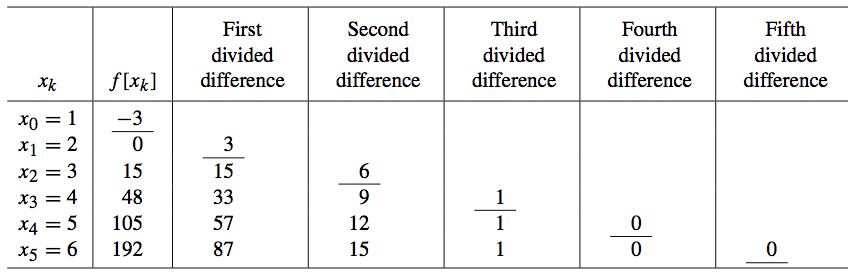
\includegraphics[width=80mm]{chap-3/tab_4-9.png}
\end{center}
\end{figure} 
%}
%\frame{
The coefficients $a_0 = -3$, $a_1 = 3$, $a_2 = 6$, and $a_3 = 1$ of $P_3(x)$ appear on the diagonal of the divided-difference table. 
The centers $x_0 = 1$, $x_2 = 2$, and $x_3 = 3$ are the values in the first column. Using formula (3.59), we write 
\begin{equation*}
P_3(x) = -3 + 3(x - 1) + 6(x - 1)(x - 2) + (x - 1)(x - 2)(x - 3).
\end{equation*} 
}

\frame{
\frametitle{Example } 
Construct a divided-difference table for $f (x) = \cos(x)$ based on the five points $(k, \cos(k))$, for $k = 0$, $1$, $2$, $3$, $4$. 
Use it to find the coefficients ak and the four Newton interpolating polynomials $P_k (x)$, for $k = 1$, $2$, $3$, $4$.
The nodes $x_0$, $x_1$, $x_2$, $x_3$ and the diagonal elements $a_0$, $a_1$, $a_2$, $a_3$, $a_4$ in the following table, and we write down the first four Newton polynomials
\begin{equation*}
\begin{array}{l c l}
P_1(x) & = & 1.0000000 - 0.4596977(x - 0.0), \\
P_2(x) & = & 1.0000000 - 0.4596977(x - 0.0) - 0.2483757(x - 0.0)(x - 1.0), \\
P_3(x) & = & 1.0000000 - 0.4596977(x - 0.0) - 0.2483757(x - 0.0)(x - 1.0) \\
& & + 0.1465592(x - 0.0)(x - 1.0)(x - 2.0), \\
P_4(x) & = & 1.0000000 - 0.4596977(x - 0.0) - 0.2483757(x - 0.0)(x - 1.0) \\
& & + 0.1465592(x - 0.0)(x - 1.0)(x - 2.0) \\
& & - 0.0146568(x - 0.0)(x - 1.0)(x - 2.0)(x - 3.0).
\end{array}
\end{equation*}
}


\frame{
\begin{figure}
\begin{center}
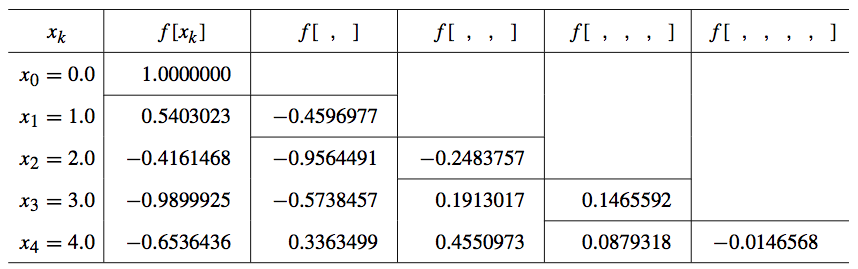
\includegraphics[width=100mm]{chap-3/tab_4-10.png}
\end{center}
\end{figure} 
The following sample calculation shows how to find the coefficient $a_2$.
\begin{equation*}
\begin{array}{l c l}
f [x_0, x_1] & = & \frac{f [x_1] - f [x_0]}{x_1 - x_0} = \frac{0.5403023 - 10000000}{1.0 - 0.0} = -0.4596977, \\
f [x_1, x_2] & = & \frac{f [x_2] - f [x_1]}{x_2 - x_1} = \frac{-0.4161468 - 0.5403023}{2.0 - 1.0} = -0.9564491,
\end{array}
\end{equation*}
\begin{equation*}
\begin{array}{l c l}
a_2 & = & f [x_0, x_1, x_2] = \frac{f [x_1, x_2] - f [x_0, x_1]}{x_2 - x_0}  \\
& = & \frac{-0.9564491+ 0.4596977}{2.0 - 0.0} = -0.2483757
\end{array}
\end{equation*}
}

\frame{
The graphs of $y = cos(x)$ and $y = P_1(x)$, $y = P_2(x)$, and $y = P_3(x)$ are shown in the following figures. 
\begin{columns}
\begin{column}{0.5\textwidth}
\begin{figure}
\begin{center}
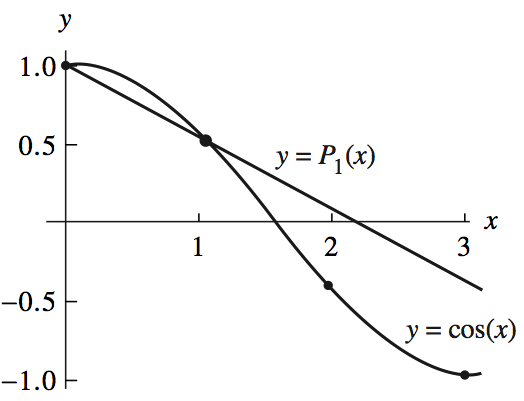
\includegraphics[width=40mm]{chap-3/fig_4-14.png}
\end{center}
\end{figure} 
\end{column}
\begin{column}{0.5\textwidth}
\begin{figure}
\begin{center}
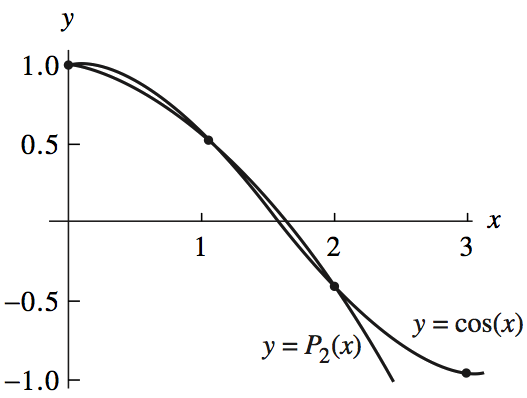
\includegraphics[width=40mm]{chap-3/fig_4-14_2.png}
\end{center}
\end{figure} 
\end{column}
\end{columns}
\begin{figure}
\begin{center}
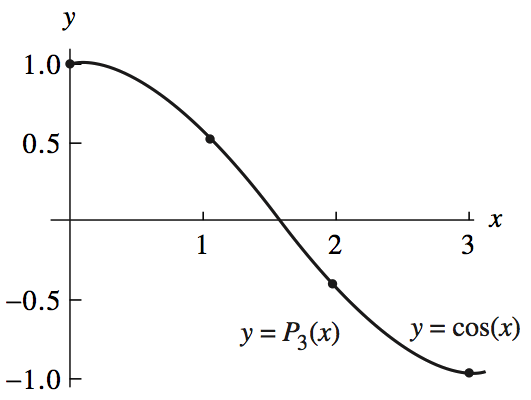
\includegraphics[width=40mm]{chap-3/fig_4-14_3.png}
\end{center}
\end{figure} 
}


\frame{
For computational purposes the divided differences in Table 3.8 need to be stored in an array which is chosen to be $D(k,j)$, so that
\begin{equation*}
D(k, j ) = f [x_{k-j} , x_{k-j+1}, \ldots, x_k ] \ \ \ for \ \  j \le k.
\end{equation*} 
Relation (3.70) is used to obtain the formula to recursively compute the entries in the array:
\begin{equation*}
D(k, j ) = \frac{ D(k, j - 1) - D(k - 1, j - 1)}{x_k - x_{k-j}}
\end{equation*} 
\begin{itemize}
\item Notice that the value ak in (3.71) is the diagonal element $a_k = D(k, k)$. 
\item The algorithm for computing the divided differences and evaluating $P_N(x)$ is now given. 
\item We remark that Problem 2 in Algorithms and Programs investigates how to modify the algorithm so that the values $\{ a_k \}$ are computed using a one-dimensional array. 
\end{itemize}
}



